\documentclass[12pt]{article}
\usepackage[margin=1in]{geometry}
\usepackage{amsmath}
\usepackage{graphicx}
\usepackage{float}
\usepackage{enumitem}
\usepackage{booktabs}
\usepackage{tikz}
\usepackage{fancyhdr}
\usepackage[rgb]{xcolor}
\usepackage{tcolorbox}
\usepackage{wrapfig}

% Define colors
\definecolor{labblue}{RGB}{51,101,138}
\definecolor{safetyyellow}{RGB}{255,240,150}

% Configure page style
\pagestyle{fancy}
\fancyhead{}
\fancyhead[L]{Physics Laboratory}
\fancyhead[R]{Newton's Second Law}
\fancyfoot{}
\fancyfoot[C]{\thepage}

\begin{document}

\begin{center}
{\Large \textbf{Laboratory Exercise E1:}}\\[0.5cm]
{\LARGE \textbf{Newton's Second Law}}\\[1cm]
\rule{\textwidth}{0.4pt}
\end{center}

\section*{Introduction}
In this laboratory exercise, you will investigate Newton's Second Law of Motion: $$\vec{F} = m\vec{a}$$
where $\vec{F}$ is the net force acting on an object, $m$ is the object's mass, and $\vec{a}$ is its acceleration.

\begin{tcolorbox}[colback=labblue!10,colframe=labblue,title=\textbf{Key Terms}]
\begin{itemize}
\item \textbf{Force}: A push or pull that can change an object's motion
\item \textbf{Mass}: The amount of matter in an object
\item \textbf{Acceleration}: The rate of change of velocity
\item \textbf{Net Force}: The total force acting on an object
\end{itemize}
\end{tcolorbox}

\section*{Objectives}
After completing this lab, you will be able to:
\begin{enumerate}[label=\arabic*.]
\item Measure the acceleration of an object under different forces
\item Create and analyze force vs. acceleration graphs
\item Use Excel to process and analyze experimental data
\item Determine an object's mass from experimental measurements
\item Evaluate experimental uncertainty
\end{enumerate}

\section*{Materials and Equipment}
\begin{itemize}
\item Dynamics cart
\item Track with pulley
\item Hanging masses 
\item Meter stick
\item Stopwatch
\item Electronic balance
\item Computer with Excel
\item String (approximately 1m)
\end{itemize}

\section*{Safety Precautions}
\begin{tcolorbox}[colback=safetyyellow!30,colframe=safetyyellow!80,title=\textbf{Safety First!}]
\begin{itemize}
\item Keep the floor area clear of obstacles
\item Secure the track properly to prevent tipping
\item Handle hanging masses carefully to avoid dropping
\item Ensure string is properly tied to prevent masses from falling
\item Keep hands clear of moving cart and pulley
\end{itemize}
\end{tcolorbox}

\section*{Experimental Setup}
\begin{center}
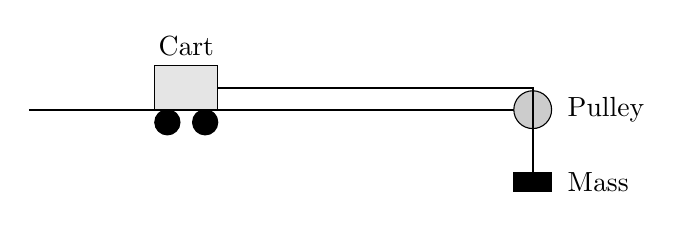
\begin{tikzpicture}[scale=0.8]
% Draw track
\draw[thick] (0,2) -- (8,2);
% Draw cart
\draw[fill=gray!20] (2,2) rectangle (3,2.7);
\draw[fill=black] (2.2,1.8) circle (0.2);
\draw[fill=black] (2.8,1.8) circle (0.2);
% Draw pulley
\draw[fill=gray!40] (8,2) circle (0.3);
% Draw string and mass
\draw[thick] (3,2.35) -- (8,2.35) -- (8,1);
\draw[fill=black] (7.7,0.7) rectangle (8.3,1);
% Labels
\node[above] at (2.5,2.7) {Cart};
\node[right] at (8.4,2) {Pulley};
\node[right] at (8.4,0.85) {Mass};
\end{tikzpicture}
\end{center}

\section*{Procedure}
\begin{enumerate}[label=\arabic*.]
\item Level the track using the adjustable feet
\item Measure and record the mass of the cart ($M_c$)
\item Attach the string to the cart and over the pulley
\item Add a 50g mass ($m$) to the hanging end
\item Mark a distance of 1.0 meter on the track
\item Release the cart from rest and measure the time to travel 1.0 meter
\item Repeat the measurement 3 times
\item Add another 50g mass and repeat steps 6-7
\item Continue until you have data for 5 different hanging masses
\end{enumerate}

\section*{Data Collection}
Record your measurements in Excel using the following table format:

\begin{table}[H]
\centering
\begin{tabular}{cccccc}
\toprule
Hanging Mass & Time 1 & Time 2 & Time 3 & Average Time & Acceleration \\
(kg) & (s) & (s) & (s) & (s) & (m/s²) \\
\midrule
0.050 & & & & & \\
0.100 & & & & & \\
0.150 & & & & & \\
0.200 & & & & & \\
0.250 & & & & & \\
\bottomrule
\end{tabular}
\end{table}

\section*{Data Analysis in Excel}
\begin{enumerate}[label=\arabic*.]
\item Calculate the average time for each mass
\begin{tcolorbox}[colback=labblue!5,colframe=labblue]
Excel Formula: \texttt{=AVERAGE(B2:D2)}
\end{tcolorbox}

\item Calculate acceleration using:
$$a = \frac{2d}{t^2}$$
where $d = 1.0$ m and $t$ is the average time.
\begin{tcolorbox}[colback=labblue!5,colframe=labblue]
Excel Formula: \texttt{=2*1/(E2\^{}2)}
\end{tcolorbox}

\item Calculate the net force for each trial:
$$F_{net} = mg$$
where $g = 9.81$ m/s²

\item Create a scatter plot of Force vs. Acceleration
\begin{enumerate}[label=\alph*.]
\item Select your force and acceleration data
\item Click Insert → Scatter Plot
\item Add axis labels and title
\item Add a trendline and display equation
\end{enumerate}

\end{enumerate}

\section*{Calculations}
The slope of your Force vs. Acceleration graph represents the mass of the cart:
$$\text{slope} = \frac{\Delta F}{\Delta a} = m$$

Calculate percent error:
$$\text{Percent Error} = \left|\frac{\text{Measured Mass} - \text{Actual Mass}}{\text{Actual Mass}}\right| \times 100\%$$

\section*{Discussion Questions}
\begin{enumerate}[label=\arabic*.]
\item How does your calculated mass compare to the measured mass of the cart?
\item What are possible sources of error in this experiment?
\item How would friction affect your results?
\item Why did we take multiple time measurements for each mass?
\item What does the y-intercept of your graph represent?
\end{enumerate}

\section*{Conclusion}
Summarize your findings by discussing:
\begin{itemize}
\item The relationship between force and acceleration
\item The accuracy of your mass determination
\item Major sources of experimental error
\item Suggestions for improving the experiment
\end{itemize}

\end{document}